
\chapter{Evaluation, Results and Discussion}
\label{ch:evaluation}

\section{Implementation Summary}
The project is a modular full-stack web app. The client is written in React and TypeScript.
The backend is FastAPI-based with a service driven architecture and schema validation. PostgreSQL is used as the
primary database and Redis-powered asynchronous task processing is used for background jobs.

\begin{table}[H]
	\centering
	\caption{Technology stack used in implementation}
	\begin{tabular}{p{2.0in}p{4.0in}}
		\toprule
		\textbf{Layer} & \textbf{Technology} \\
		\midruleView & React, TypeScript, Vite, TanStack Query, Zustand \\Backend & Python, FastAPI, Pydantic, JWT authenticationDatabase & PostgreSQL, SQLAlchemy async
		Frontend        & React, TypeScript, Vite, TanStack Query, Zustand \\
		Backend         & Python, FastAPI, Pydantic, JWT-based authentication \\
		Database        & PostgreSQL, SQLAlchemy async \\
		Queue / Async & Redis asynchronous tasks with workers\\
		AI Integration & Integration of local model and retrieval-augmented tutor flows \\Deployment & Local deployment with Docker Compose \\\
		Deployment      & Docker Compose based local deployment \\
		\bottomrule
	\end{tabular}
\end{table}

\section{Module-Wise Implementation}

\begin{figure}[H]
	\centering
	\begin{tikzpicture}[
		node distance=7mm and 8mm,
		m/.style={draw, rounded corners, align=center, minimum width=2.6cm, minimum height=8mm, fill=kuetgray},
		arr/.style={-{Stealth}, thick}
		]
		\node[m, fill=blue!10] (auth) {Auth + Profile};
		\node[m, right=of auth, fill=blue!10] (courses) {Courses + Topics};
		\node[m, below=of courses, fill=blue!10] (routine) {Routine + Attendance};
		\node[m, below=of auth, fill=green!10] (tutor) {AI Tutor};
		\node[m, below=of courses, fill=green!10] (community) {Community};
		\node[m, below=of routine, fill=green!10] (notif) {Notifications};
		\node[m, below=of community, fill=orange!12] (analytics) {Analytics};
		
		\draw[arr] (auth) -- (courses);
		\draw[arr] (courses) -- (routine);
		\draw[arr] (courses) -- (tutor);
		\draw[arr] (community) -- (notif);
		\draw[arr] (routine) -- (analytics);
		\draw[arr] (tutor) -- (analytics);
		\draw[arr] (community) -- (analytics);
	\end{tikzpicture}
	\caption{Module connectivity in implementation.}
	\label{fig:module-connectivity}
\end{figure}

\subsection{Authentication and Profile}
Token-based authentication is used. Secured resources use backend dependencies to
authorized access. Profile operations include: user details, avatar and account.
operations.

\subsection{Course and Topic Management}
Course management includes list, detail, data based on enrollments, topic actions and material actions. The
There are route and service layers connecting the front-end with the back-end for consistent CRUD operations.

\subsection{AI Tutor Workspace}
The AI Tutor is implemented as a multi-mode workspace for user interactions via chat,
quiz, and resources. Switching modes, maintaining topic and state in frontend
components and endpoints.

\subsection{Routine and Attendance}
Routine management covers schedule slot management and routine visualisation in the frontend. Attendance
data is included in analytics and class processes.

\subsection{Community and Classroom Operations}
Community implementation provides classrooms, threads, replies, announcements, attendance views, marks views and member
management interactions. Interaction pathways (tutor and student) are distinguished using role-based UI and checks.

\subsection{Notifications}
The notifications module includes listing, unread counts, mark as read, and response actions for classes.
Realtime updates are linked to frontend state management to provide realtime visual feedback.

\subsection{Analytics Dashboard}
Analytics offers an overview and per-course view. It is connected with attendance and scoring entities,
with two perspectives for student and tutors.

\section{API Implementation Snapshot}
\begin{table}[H]
	\centering
	\caption{Some API Endpoints implemented}
	\begin{tabular}{p{1.5in}p{2.5in}p{2.0in}}
		\toprule
		\textbf{Module} & \textbf{Endpoint} & \textbf{Purpose} \\
		\midruleAuth & /api/auth/* & Account and authentication \\Courses & /api/courses/* & Course, topic and material management \\Routine & /api/routine/* & Routine and slot flows \\AI Tutor & /api/ai-tutor/* & Multimodal tutor flows \\
		Auth          & /api/auth/*                     & Authentication and account flows \\
		Courses       & /api/courses/*                  & Course, topic, and material operations \\
		Routine       & /api/routine/*                  & Routine and slot-related operations \\
		AI Tutor      & /api/ai-tutor/*                 & Multi-mode tutor interactions \\
		Community & /api/community/* & Classroom, thread and announcement flows \\nouncement flows \\
		Notifications & /api/notifications/* & Notification and response actions \\ actions \\
		Analytics & /api/analytics/* & Overview and course analytics \\Profile & /api/profile/* & User profile and account \\Settings & /api/settings/* & User preferences and settings \\course analytics \\
		Profile       & /api/profile/*                  & Profile and account management \\
		Settings      & /api/settings/*                 & User preferences and settings \\
		\bottomrule
	\end{tabular}
\end{table}

\section{User Interface}
The user interface (UI) is based on dedicated pages for each project core module. The screenshots below are the major
user interfaces implemented in the system.

\begin{figure}[H]
	\centering
	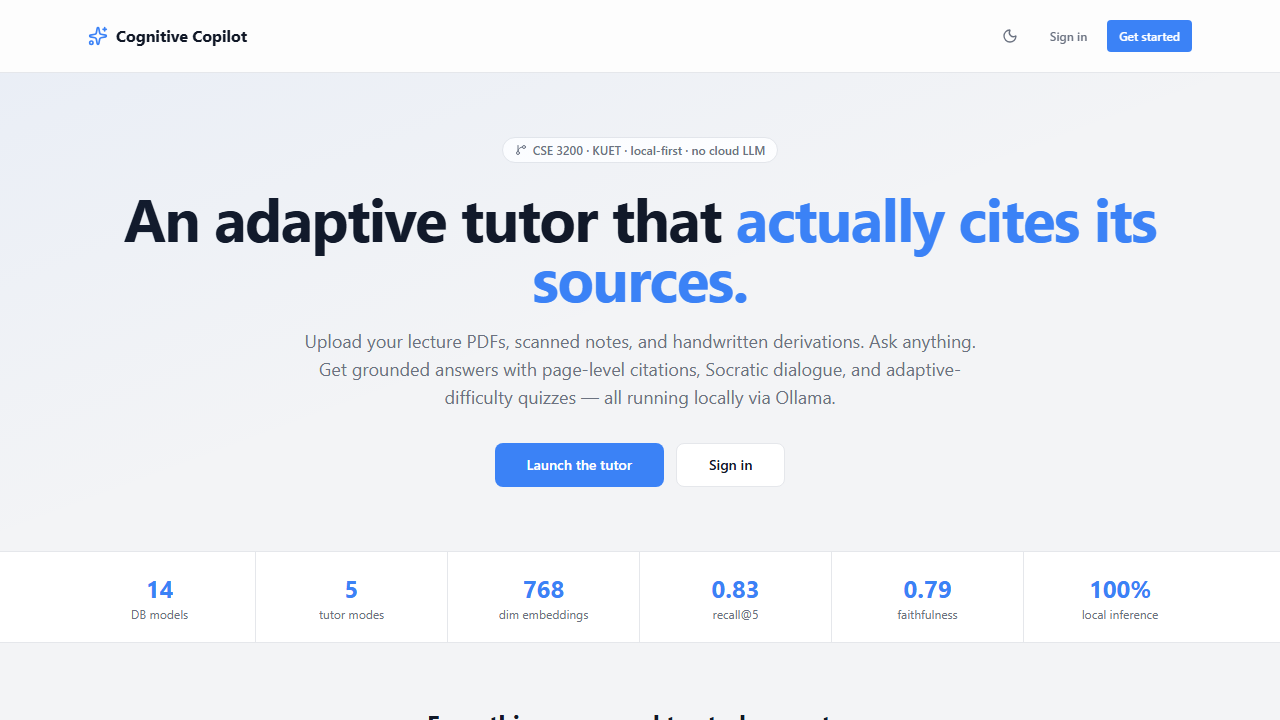
\includegraphics[width=0.95\textwidth]{assets/screenshots/landing.png}
	\caption{Landing Page}
\end{figure}

\begin{figure}[H]
	\centering
	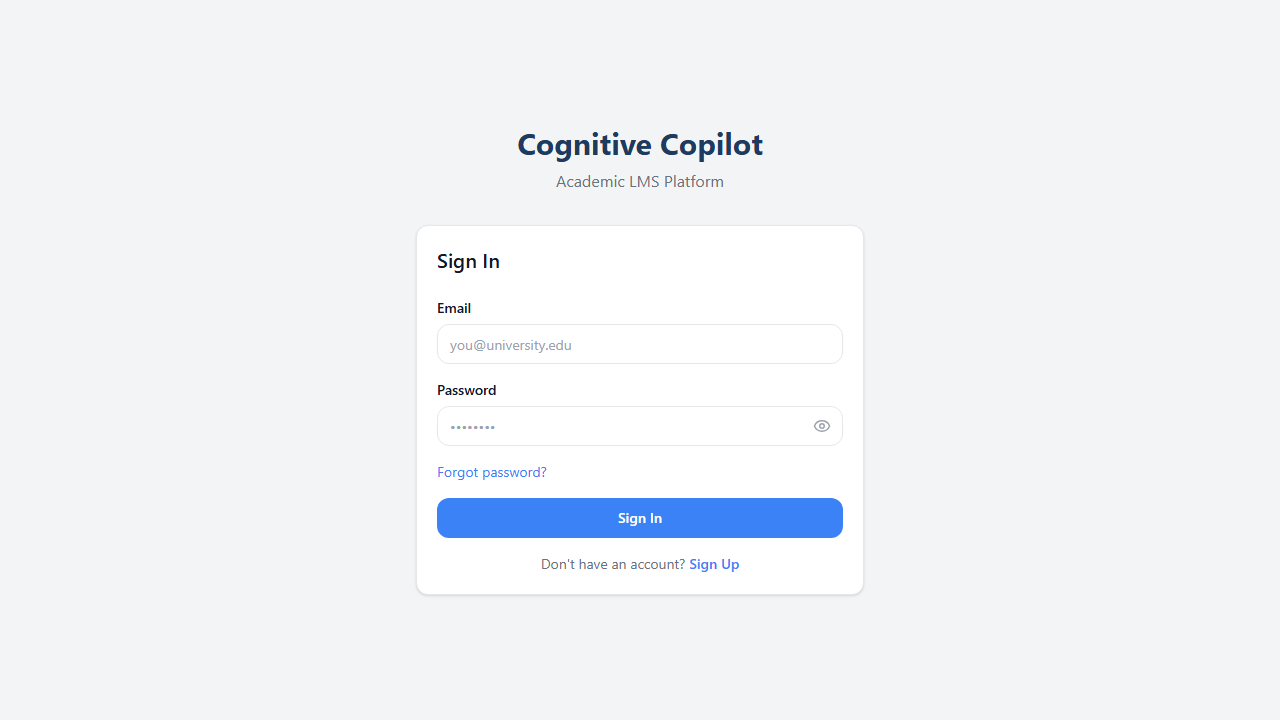
\includegraphics[width=0.95\textwidth]{assets/screenshots/login.png}
	\caption{Login Interface}
\end{figure}

\begin{figure}[H]
	\centering
	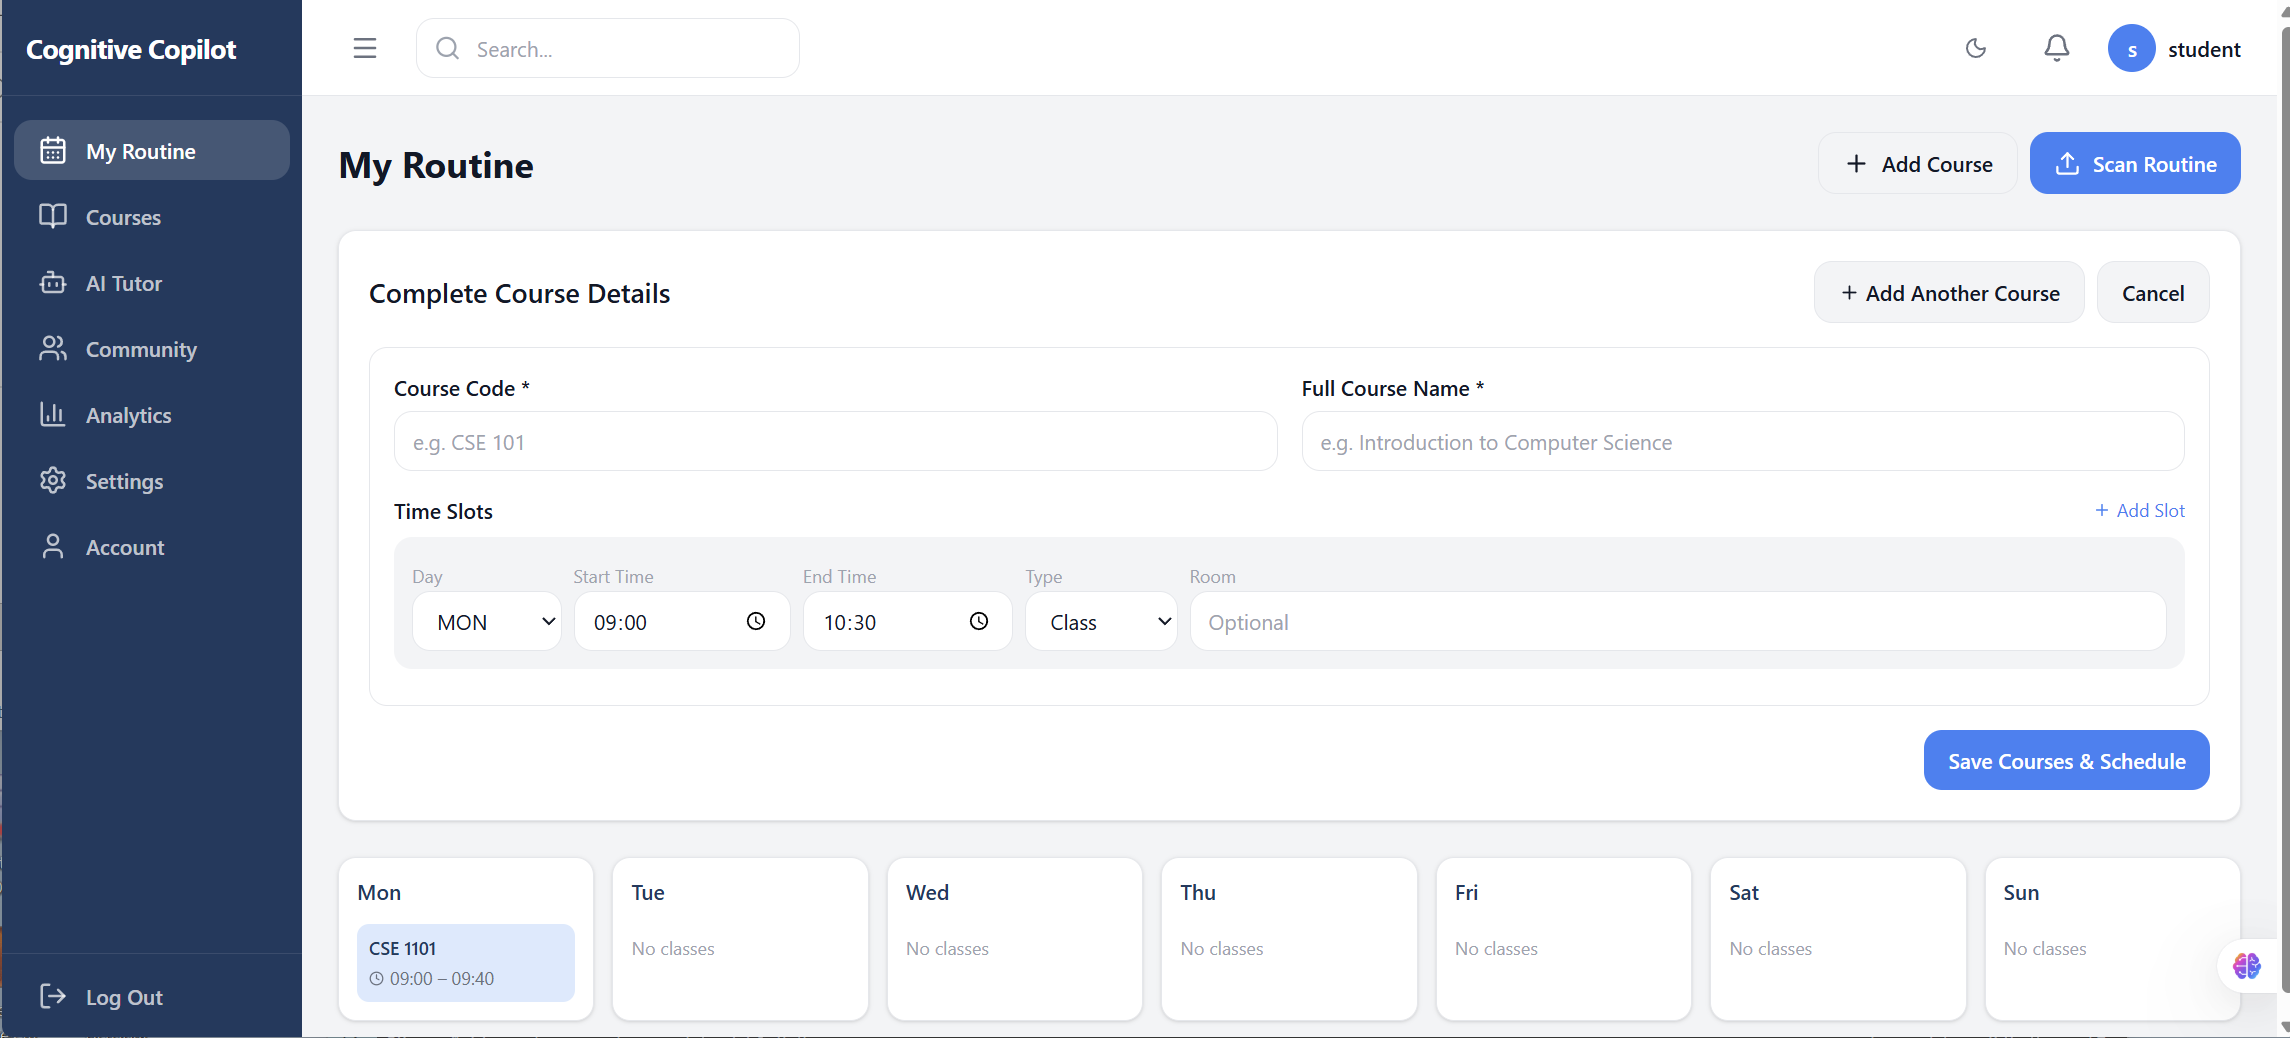
\includegraphics[width=0.95\textwidth]{assets/screenshots/routine.png}
	\caption{View of Routine Page and Slot}
\end{figure}

\begin{figure}[H]
	\centering
	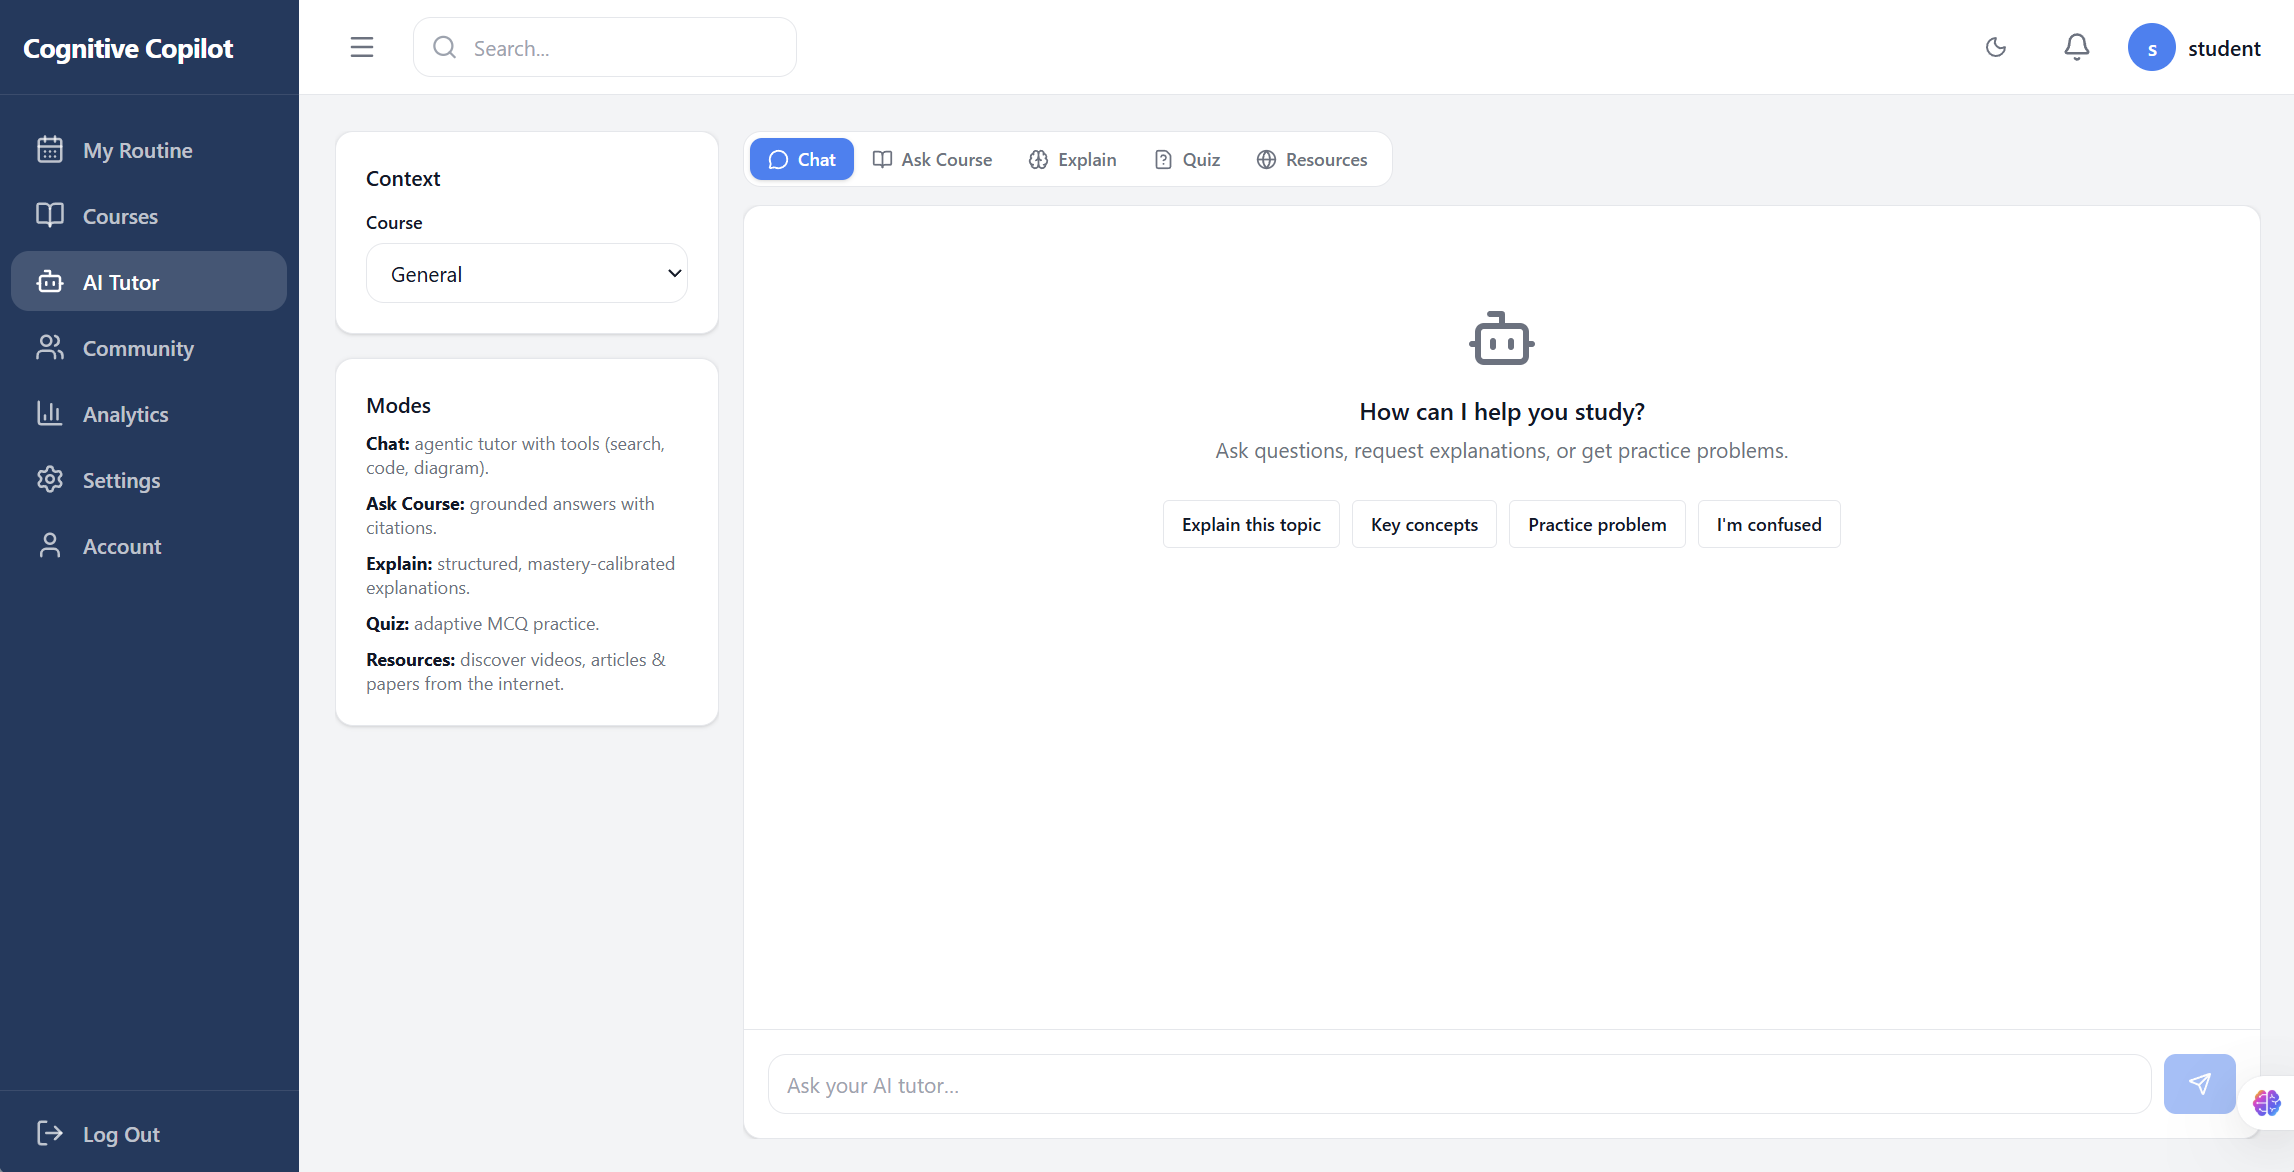
\includegraphics[width=0.95\textwidth]{assets/screenshots/ai_tutor.png}
	\caption{AI Tutor Workspace}
\end{figure}

\begin{figure}[H]
	\centering
	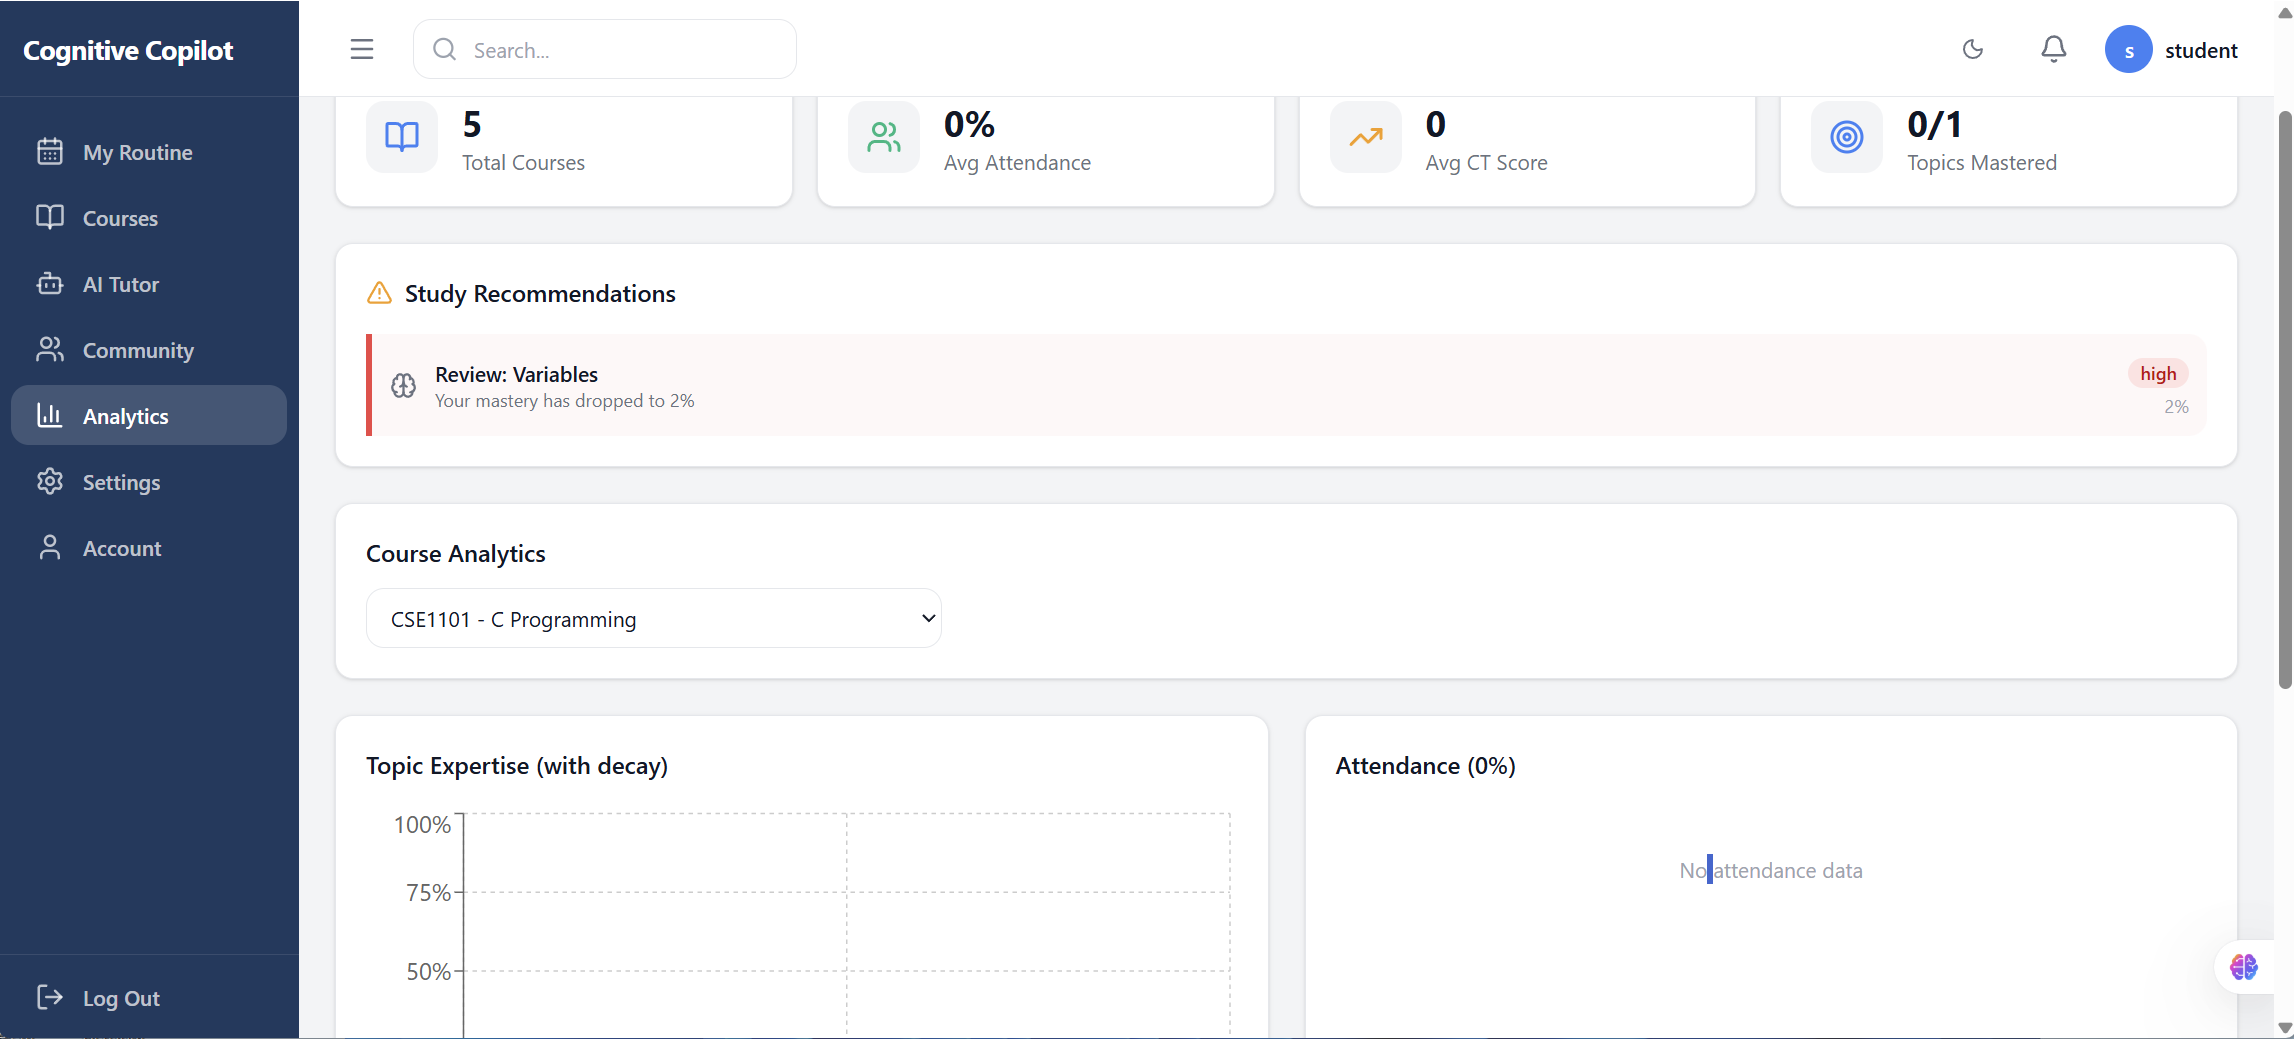
\includegraphics[width=0.95\textwidth]{assets/screenshots/analytics.png}
	\caption{Analytics Dashboard}
\end{figure}

\begin{figure}[H]
	\centering
	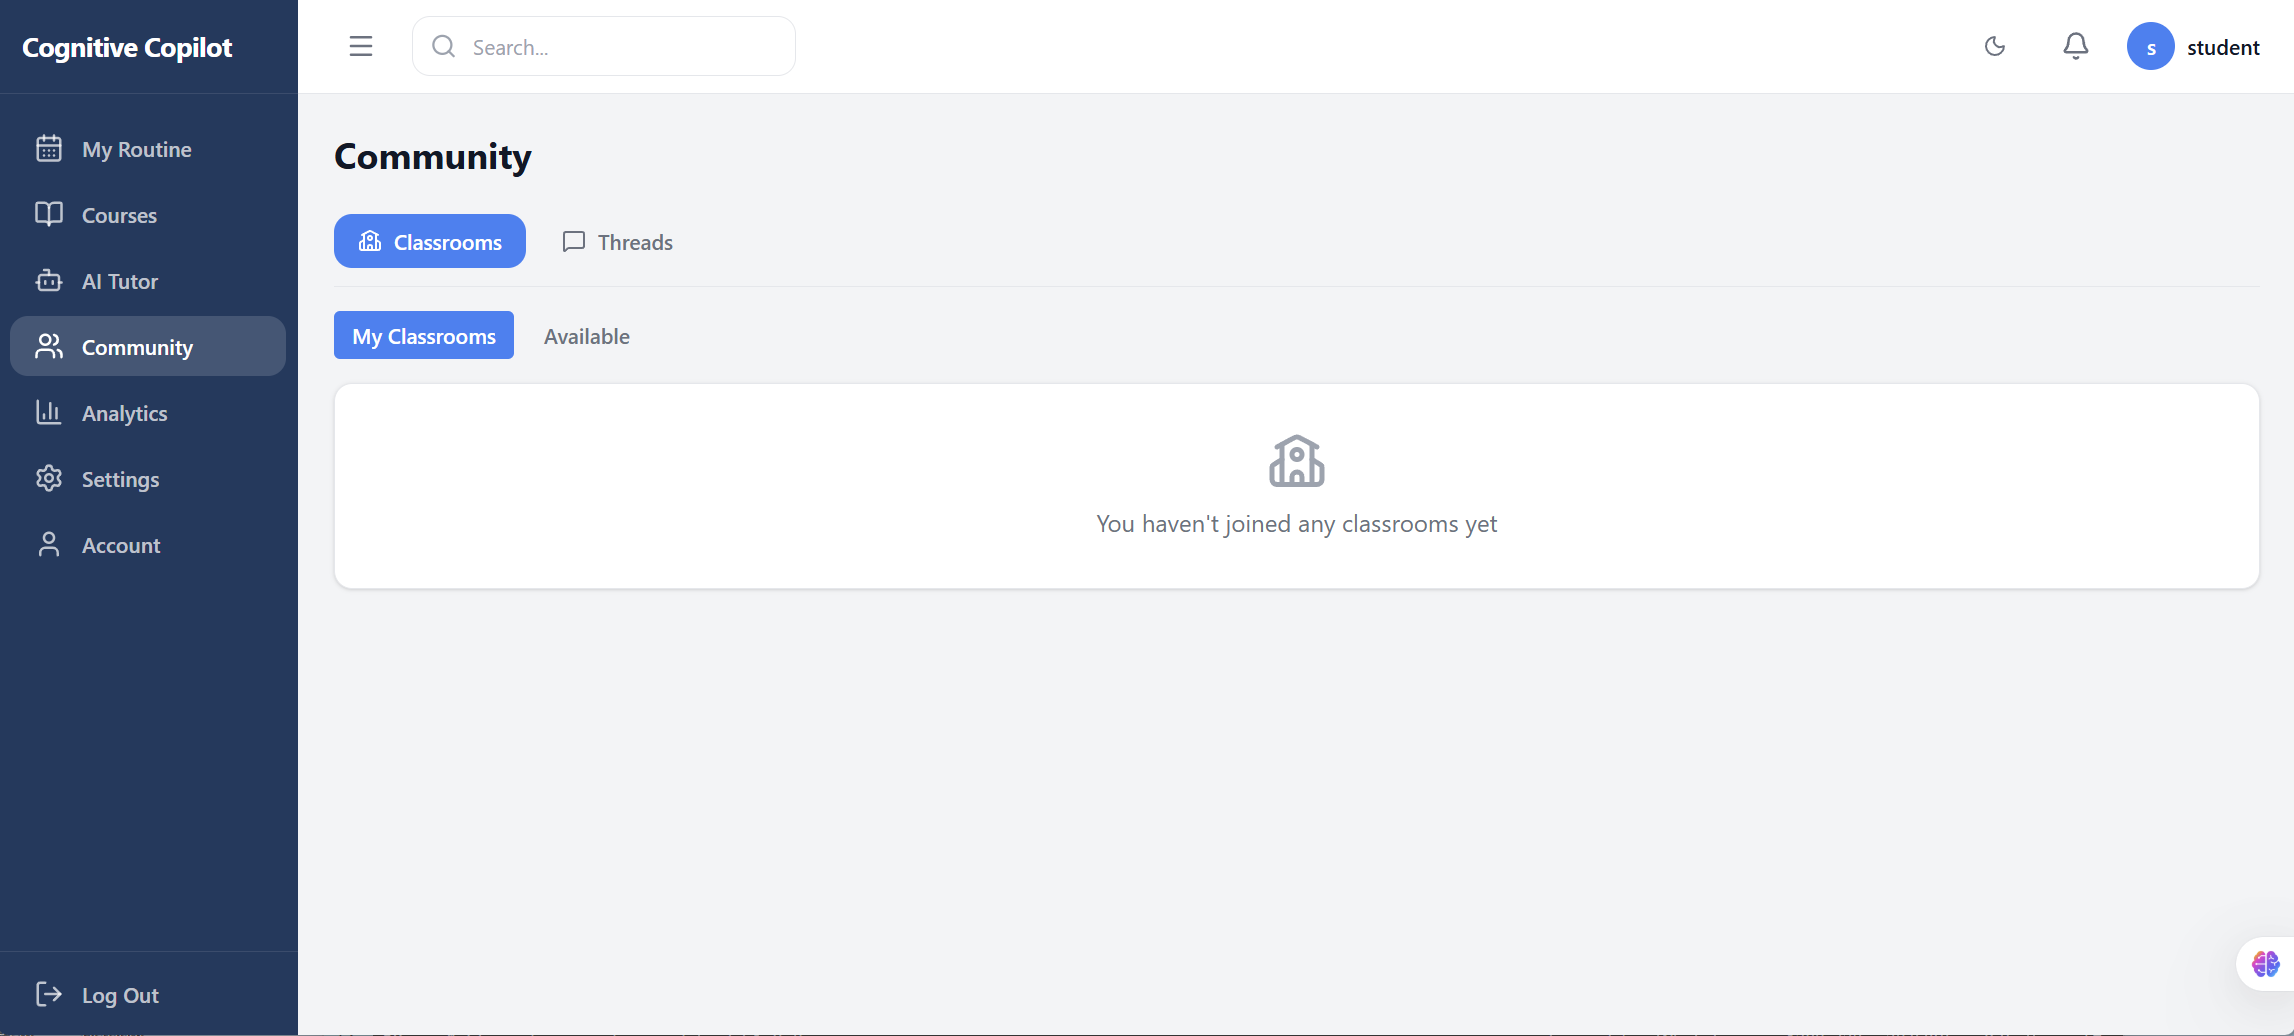
\includegraphics[width=0.95\textwidth]{assets/screenshots/community.png}
	\caption{Community and Classroom Flow}
\end{figure}

\begin{figure}[H]
	\centering
	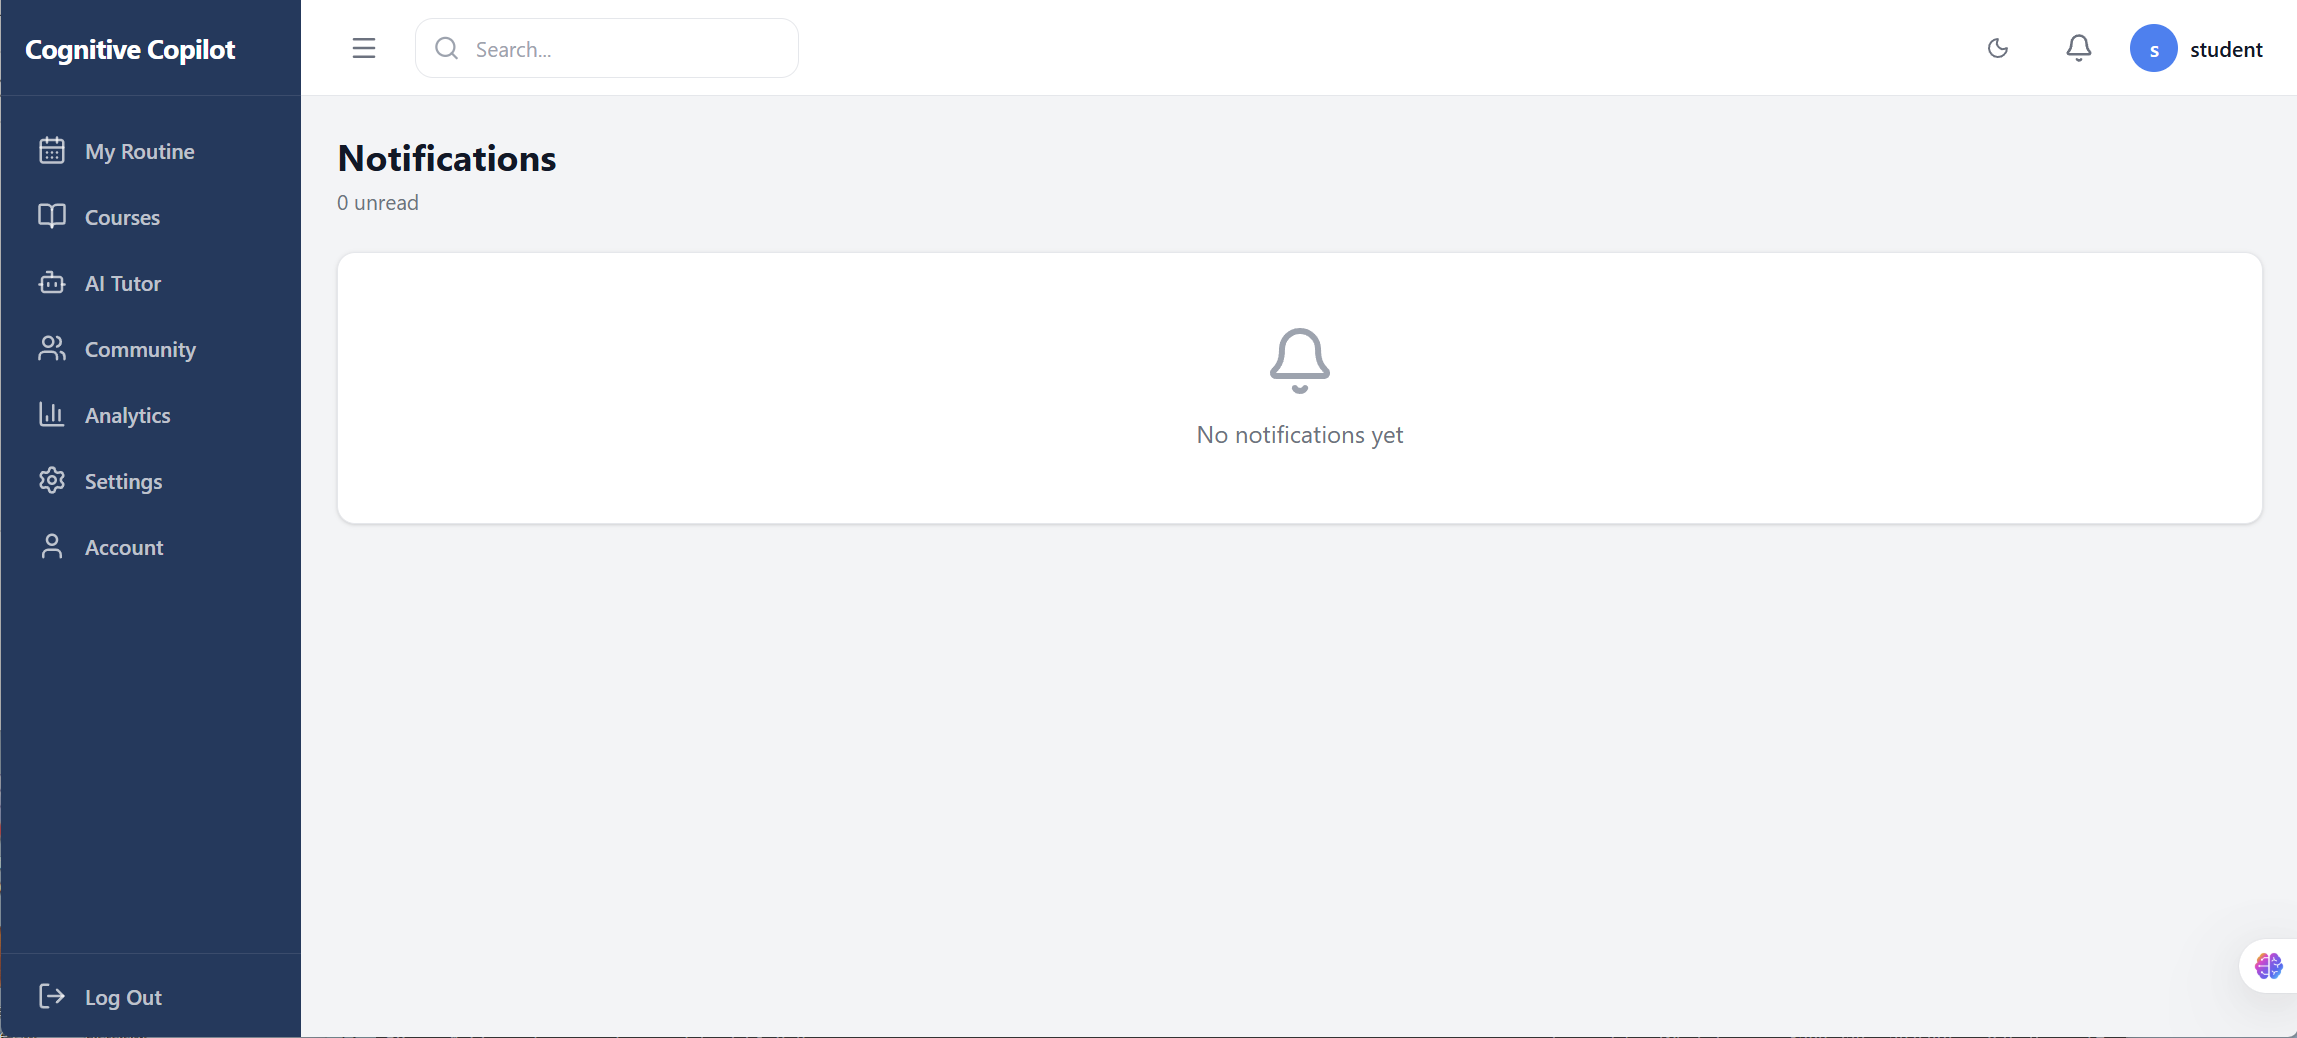
\includegraphics[width=0.95\textwidth]{assets/screenshots/notifications.png}
	\caption{Notification Center with Deep-links}
\end{figure}

\section{Discussion}
This project shows that a system can integrate wide-ranging academic processes with AI-driven learning.
maintainable system. The key engineering success is consistency: the user works with linked modules
rather than separate apps, and the code is well-organised into route-service-data.

The project also illustrates the trade-offs. AI features enhance user experience and research, but they need to be
need to be complemented by sound CRUD and authorization. As a consequence, the implementation and testing concentrate on
correct interactions, API contracts and module integration instead of untested benchmark claims.